\chapter{Auctions}
\label{ch:auctions}
\index{auctions}

Auctions are a common and simple way of performing resource allocation
in a multiagent system. In an auction, agents can express how much
they want a particular item via their bid and a central auctioneer can
make the allocation based on these bids. Of course, this generally
requires the use of a centralized auctioneer but there are techniques
for reducing this bottleneck. Still, even centralized auctions can be
very complex and produce unexpected results if one does not understand
all the details.

\section{Valuations}
\label{sec:valuations}

Before we begin to talk about the various types of auctions we must
first clarify how people value the items being sold. We have used the
notation $u_i(s)$ to refer to the utility that agent $i$ derives from
state $s$. Similarly, if $s$ is instead an item, or set of items, for
sale we can say that $v_i(s)$ is the \td{valuation} that $i$ assigns
to $s$.  We furthermore assume that this valuation is expressed in a
common currency, thus $v_i(s)$ then becomes the maximum amount of
money that agent $i$ is willing to pay for $s$. When studying auctions
we generally assume that all agents have a valuation function over all
the items being sold.

In the simplest case this valuation function reflects the agent's
utility of owning the given items. For example, if you plan to eat a
meal then the amount you are willing to pay for each item in the menu
depends solely on how hungry you are and how much you like each item.
In these cases we say that the agent has a \td{private value}
function.

On the other hand, there are items which you cannot consume and gain
no direct utility from but which might still have a resale value. The
classic example are stocks. When you buy a share in some company you
cannot do anything with that share, except sell it. As such, your
valuation on that share depends completely on the value that others
attribute, and will attribute, to that share. These are known as
\td{common value} functions.

Most cases, however, lie somewhere in the middle. When you buy a house
you take into consideration the value that you will derive from living
in that house as well as its appreciation prospects: the price you
think others will pay when you finally sell it. This is an example of
a \td{correlated value} function and is very common in the real world
with durable high priced items.

The type of valuation function that the agents use changes their
optimal behavior in an auction. For example, if an agent has a common
value function then it will likely pay more attention to what the
other agents are bidding. Most multiagent implementations use agents
with private value functions as most systems do not want to waste the
time required to implement secondary markets for the items being sold.
Still, in open multiagent systems it might be impossible to prevent
secondary markets from appearing.


\section{Simple Auctions}

There are times when there are many agents and the only thing they
need to negotiate over is price. In these occasions it makes sense to
use an auction since they are fast and require little agent
communication. However, auctions are not as simple as they might
appear at first and there are many ways in which things can go wrong
when using them.

The actual mechanisms used for carrying out an auction are varied. The
most common of all is the \td{English auction}. This is a
\td{first-price open-cry ascending} auction.  It is the standard one
used in most auction houses. In it, the auctioneer raises the price as
people yell higher bids. Once no one is willing to bid higher, the
person with the highest bid gets the item and pays his bid price.
These auctions sometimes have an initial or \td{reservation price}
below which the seller is not willing to sell. The dominant strategy
in an English auction, with private value, is to bid the current price
plus some small amount until either the auction is won or one's
reservation price is reached.

If an English auction is common or correlated value then it suffers
from the \td{winner's curse}. For example, when you buy a stock in an
English auction it means that you paid more than anyone else was
willing to pay. As such, your valuation of that share must now be less
than what you paid for it. In the real world we gamble that at some
point in the future the others will realize that this stock really is
worth that much more.
\medskip

A similar auction type is the \td{First-price sealed-bid} auction. In
this auction each person places his bid in a sealed envelope. These
are given to the auctioneer who then picks the highest bid. The winner
must pay his bid amount.  These auctions have no dominant strategy.
The buyer's best strategy is to spy on the other bidders in order to
determine what they are going to bid and then bid slightly higher than
that, as long as that is less than one's reservation price. If spying
is impossible then the agent has no clearly superior strategy.
Because of the incentive for spying, these auctions lead to a lot of
inefficiencies when paired with intelligent agents.

\medskip

\mc{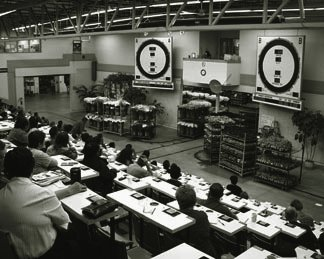
\includegraphics[width=\marginparwidth]{auctions/flowermarket}
  Ontario Flower Growers Co-op, an example of a Dutch auction at work.
  The two large circles in the back are used to show the descending
  price.}

The \td{Dutch} auction is an \td{open-cry descending price} auction.
In it the seller continuously lowers the selling price until a buyer
hits a buzzer, agreeing to buy at the current price. The auction's
name comes from its use by the Dutch to sell flowers. The Dutch flower
markets have been around for centuries and are still thriving. Every
morning carts of flowers are paraded before eager flower shop owners
who are equipped with a buzzer. Each cart stops before the buyers and
a clock starts ticking backwards from a high number. When the first
buyer hits his buzzer the flowers are sold to him at the current
price. Analysis of the Dutch auction shows that it is equivalent to a
first-price sealed-bid auction in terms of strategy. That is, it has
no dominant strategy. However, it has the nice property of being
real-time efficient. The auction closes quickly and the auctioneer can
make it move even faster by lowering the price faster.  This real-time
efficiency makes it a very attractive auction for selling cut flowers
as these lose their value quickly after being harvested.

\medskip

%\begin{figure}
%  \begin{center}
%    \includegraphics[width=.4\textwidth]{google}
%  \end{center}  
%  \caption{A visual explanation of the Google IPO auction, from the New York Times.}
%  \label{fig:google}
%\end{figure}

%A few years ago Google utilized a variation on the Dutch auction to
%determine the initial price for their shares. They asked all buyers to
%submit their bids. Each bid contained the number of shares and the
%price per share the buyer was willing to pay. They then sorted all
%these and, starting from the highest bids, counted backwards until
%they had sold all their shares. The price that they sold at was given
%by the last price price they counted (that is, the smallest price).
%The method is nicely summarized by the graph shown in
%Figure~\ref{fig:google}. It seems to me, however, that the Google
%auction was more similar to a Vickrey auction than to a Dutch auction.
%I don't understand why they called it a Dutch auction. 

The \td{Vickrey} auction is a more recent addition and has some very
interesting properties. It is a \td{second-price sealed-bid} auction.
All agents place their bids and the agent with the highest bid wins
the auction but the price he pays is the price of the second highest
bid. Analysis of this auction has shown that bidding one's true
valuation, in a private value auction, is the dominant strategy. For
example, let your valuation for the item being sold be $v$.  If you
bid less than $v$ then you are risking the possibility that some other
agent will bid $w < v$ and get the item even though you could have won
it.  Moreover, since $w$ is less than $v$ you could have bid $v$ and
paid only $w$.  As such, you have nothing to gain by bidding less than
$v$ but risk the possibility of losing an auction that you could have
won at an acceptable price. On the other hand, if you bid $v' > v$
then you are risking that some other agent will bid $w$, where $v'> w
> v$, and thereby cause you to pay more than your reservation price
$v$. At the same time, you do not gain anything by bidding higher than
$v$ because the only auction that you might win by bidding $v'$
instead of $v$ are those where you have to pay more than $v$.

\mpic{auctions/vickrey}{William Vickrey}{1914}{1996}{Nobel Prize in
  Economics.} As such, the Vickrey auction eliminates the need for
strategizing.  Since there is an easy dominant strategy the agents do
not have to think about what they should do. They just play their
dominant strategy and bid their true valuation. Thus makes it a very
attractive auction in terms of its efficiency but it is also for this
reason that most people don't like Vickrey auctions. People are often
hesitant about revealing their true valuations for an item because we
know that the world is an iterated game and this information could be
used against us in some future auction. As such, Vickrey auctions are
seldom used in the real world.  \medskip

Finally, the \td{double auction} is a way of selling multiple units of
the same item. It is the auction used in stock markets. Each buyer
places either a buy or a sell order at a particular price for a number
of instances of the item (number of shares in the stock-market). The
buy and sell bids can be visualized in a simple graph such as the one
shown in Figure~\ref{fig:double}. Here, the $x$-axis represents a
price and each box represents an offer to buy or sell a share at the
given price.

\begin{SCfigure}
  \begin{minipage}{1.0\linewidth}
    \begin{center}
      \begin{tikzpicture}[style=dstyle,minimum size=.8cm]
        \draw[|->] (.4,0) -- (6.1,0);

        \node at (1,-2.5)[color=gray] {\textcolor{black}{1}};
        \node at (2,-2.5)[color=gray] {\textcolor{black}{2}};
        \node at (3,-2.5)[color=gray] {\textcolor{black}{3}};
        \node at (4,-2.5)[color=gray] {\textcolor{black}{4}};
        \node at (5,-2.5)[color=gray] {\textcolor{black}{5}};
        
        \node (s1) at (1,.5)[draw] {Sell};
        \node (s2) at (1,1.5)[draw] {Sell};
        \node (s3) at (2,.5)[draw] {Sell};
        \node (s4) at (3,.5)[draw] {Sell};
        \node (s5) at (5,.5)[draw] {Sell};

        \node (b1) at (1,-.5)[draw,color=gray] {\textcolor{black}{Buy}};
        \node (b2) at (2,-.5)[draw,color=gray] {\textcolor{black}{Buy}};
        \node (b3) at (2,-1.5)[draw,color=gray] {\textcolor{black}{Buy}};
        \node (b4) at (3,-.5)[draw,color=gray] {\textcolor{black}{Buy}};
        \node (b5) at (4,-.5)[draw,color=gray] {\textcolor{black}{Buy}};

        % \only<2>{
        %   \draw (s1) -- (b1);
        %   \draw (s2) -- (b2);
        %   \draw (s3) -- (b3);
        %   \draw (s4) -- (b4);}

        % \only<3>{
        %   \draw (s1) -- (b5);
        %   \draw (s2) -- (b4);
        %   \draw (s3) -- (b3);}
        
      \end{tikzpicture}
    \end{center}
  \end{minipage}
  \caption{Graphical representation of a double auction. The
    $x$-axis represents prices. Each box represents one buy or sell
    order at the given price.}
  \label{fig:double}
\end{SCfigure}

Once we have all the bids then it is time to clear the auction.  There
are many different ways to clear a double auction. For example, if
figure~\ref{fig:double} we could match the sell order for 1 with the
buy for 5 then pocket the difference of $5 - 1 = 4$ for ourselves, or
we could clear it at 3 and thus give both bidders a deal, or we could
match the seller for 1 with the buy for 1, and so on. As can be seen,
there are many different ways to match up these pairs and it is not
clear which one is better.

One metric we might wish to maximize is the amount of surplus, known
as the spread by traders. That is, the sum of the differences between
the buy bids and the sell bids. In some auctions this surplus is kept
by the auctioneer who then has an incentive to maximize it. Another
option is to use it to enable more bids to clear.  In the example
above the total supply and demands are 12, therefore all bids should
clear. One way to do this is to pair up all the small sell bids and
give these sellers exactly what they asked for then give the surplus
to the sell bid of 5 in order to clear it with the remaining buy bid.

Another metric we could use is a uniform price. That is, rather than
giving each seller and buyer the exact price they asked for, we give
them all one uniform clearing price. Clearly, the only buy bids that
will clear are those that are above the clearing price and the only
sell bids that clear are those below the clearing price.

\subsection{Analysis}

Now that we know the various auction types, there is an obvious
question that we must ask ourselves. On which auction do sellers make
more money? This question is answered by the following theorem.

\begin{theorem}[Revenue Equivalence]
  \label{th:revenue-eq}
  All four single-item auctions produce the same expected revenue in
  private value auctions with bidders that are risk-neutral.
\end{theorem}

We also know that if the bidders are risk-averse then the Dutch and
first-price are better.  A risk-averse bidder is willing to pay a bit
more than their private valuation in order to get the item. In a Dutch
or First-price auction a risk-averse agent can insure himself by
bidding more than would be required.

In common or correlated value cases the English auction gives a higher
revenue to the seller.  The increasing price causes others to increase
valuation.  That is, once the agent sees others bidding very high for
the item the agent realizes that the item is really worth more to the
other agents so it also raises its valuation of the item.\footnote{An
  interesting example of this was a British auction for 3G bandwidth
  licenses. The standard English auction was modified so that everyone
  must agree to buy at the current price or leave the room. This led
  to the licenses selling for 1000 times the expected amount
  \cite{harford05a}.}
\medskip

As it is often the case when money is involved, we have to be on the
look out for ways in which the agents might cheat. The problem of
\td{bidder collusion} affects all 4 auctions. In bidder collusion the
bidders come to an a-priory agreement about what they will bid.  They
determine which one of them has the higher valuation and then all the
other bidders refrain from bidding their true valuation so that the
one agent can get it for a much lower price. The winner will then need
to payback the others. The English and Vickrey auctions are especially
vulnerable to bidder collusion as they \td{self-enforce collusion}
agreements. For example, say there are 10 buyers and they realize that
one of them has a valuation of 100 while the others have a valuation
of 50 for the item. They agree to let him buy it for 1. In an English
auction one of the 99 agents could defect and bid 2. However, this
would only make the high-valuation agent bid 3, and so on until they
get to 51. The high-valuation agent will get the item for 51 so the
other agent gets nothing by defecting. The same logic applies in a
Vickrey auction.

Another problem might be that a \td{lying auctioneer} can make money
from a Vickrey auction. All he has to do is to report a higher
second-price than the one that was announced. The winner then pays
this higher second price to the auctioneer who gives the buyer the
real second price and pockets the difference. This requires that the
bids are not revealed and that the buyer does not pay the seller
directly. If the buyer paid the seller directly then a lying
auctioneer and the seller could collude to charge the buyer a higher
price. A lying auctioneer can also place a \mc{\textbf{shill}: a decoy
  who acts as an enthusiastic customer in order to stimulate the
  participation of others.} shill in an English auction. That is,
assuming that the auctioneer gets paid a percentage of the sales
price. If the auctioneer gets paid a fixed amount then there is no
incentive for him to increase the sales price.
\medskip 

When auctioning items in a series when their valuations are
interrelated, such as chairs in a dining set or bandwidth rights in
adjacent counties, it is possible to arrive at inefficient
allocations. For example, the problem in Table~\ref{tab:inef} leads to
an inefficient allocation if we first auction $t_1$ and then $t_2$.
Specifically, if we auction $t_1$ first then Agent 2 will get it as it
has the lower cost. When we then auction $t_2$ both agents have the
same cost (1) but, no matter who gets it the total cost is 2.5. If, on
the other hand agent 1 had won both tasks then the total cost would be
2.  matter who gets it the total cost is 2.5. This is the problem of
\td{inefficient allocation}.

\begin{SCtable}
  \begin{minipage}{1.0\linewidth}
    \begin{center}
      Costs of Doing Tasks
      \begin{tabular}{ccc}\toprule
        tasks&Agent 1&Agent 2\\ \midrule
        $t_1$&2&1.5\\ 
        $t_2$&1&1.5\\ 
        $t_1$,$t_2$&2&2.5\\ \bottomrule
      \end{tabular}
    \end{center}
  \end{minipage}
  \caption{Example of inefficient allocation.}
  \label{tab:inef}
\end{SCtable}

We could solve this problem if we made the agents use full lookahead
effectively building an extended-form game from their possible
interactions. With full lookahead the agents can build a tree where
each level corresponds to a task being auctioned.  In this way agent 1
can see that it will only cost him 2 to do $t_1$ and $t_2$ so it can
reduce its cost for $t_1$ from 2 to 1. Of course, this puts agent 1 at
risk of not getting $t_2$ since agent 1 generally will not know agent
2's cost for t2 so it does not know if it will win that auction.
Another much better way of solving the problem of inefficient
allocations is to use a combinatorial auction, which we will learn
about in Section~\ref{sec:ca}.

\subsection{Auction Design}

When designing an auction for a multiagent system you must make many
decisions. You must first determine what kind of control you have over
the system. It is possible that you control only the bidding agent and
the auction is already implemented, as when building agents to bid on
Ebay. It is possible that you control only the auction mechanism, as
when building an auction website. Finally, it is possible that you
might control both agents and mechanism, as when building a closed
multiagent system.

The case where you control the mechanism is especially interesting.
You must then decide what bidding rules you will use: when bids are to
be placed, when they can no longer be placed, what form can these bids
takes, and what rules they must follow. For example, you might set a
rule that a new bid has to always be for a higher value. You also set
up clearing rules which determine when the items are sold. We
explained some of the problems with various clearing rules in the
double auction. The four standard auction types already have clearing
rules but you might want to modify these. Finally, you must decide on
information rules: how much information the agents are to know about
what the other agents bid, whether to reveal information during the
bidding process itself or after clearing \cite{wurman02a}.

Currently all online auctions are implemented as centralized web
applications but it is not hard to imagine a future where the auctions
are freed from the constraints of a central hub and become a protocol
enacted by buying and selling agents.

\section{Combinatorial Auctions}
\label{sec:ca}

Arguably, the \td{combinatorial auction} has been the most widely used
auction in multiagent systems. In it agents can place bids for sets of
items instead of just placing one bid for each item for sale. In many
systems we have the problem that there is a set of tasks or jobs that
needs to be distributed among the agents but the agents have complex
preferences over the set of tasks. For example, in a workflow
application we have a set of workflows, each composed of a set of web
services, which must be performed by certain deadlines.  Each agent
can perform a subset of the services but each agent has different
costs which might depend on the agent's type, its current load, the
services it has done before, etc. Our problem as system designers is
to allocate the workflows to agents so that we maximize the total
number of workflows completed. Another example of combinatorial
auctions is the selling of broadcasting rights by the federal
government where cellular companies prefer to own the same frequencies
in nearby locations, or at least to own some bandwidth in all the
neighborhoods of a city. A final example is the buying of parts to put
together a PC which requires a motherboard, CPU, ram, etc.  Each part
can be bought independently but only some bundles work together.
These problems, and all problems of this type, can be solved by a
combinatorial auction.

Formally, we define a combinatorial auction over a set of items $M$ as
being composed of a set of bids, where each agent can supply many
different bids for different subset of items. Each bid $b \in B$ is
composed of \bidi{}, which is the set of items the bid is over,
\bidv{} the value or price of the bid, and \bida{} which is the agent
that placed the bid.

\pgfdeclareimage[interpolate=true,width=6cm]{titans}{auctions/teentitansf}

\begin{SCfigure}
  \begin{minipage}{1.0\linewidth}
    \begin{center}
      \begin{tikzpicture}[style=dstyle]
        \pgftext[at=\pgfpoint{-3cm}{0cm}]{\pgfuseimage{titans}};
        \node at (3,0) {
          \begin{tabular}{lc}\toprule
            Price &Bid items  \\ \midrule
            \$$1$  &Beast Boy \\ 
            \$$3$  &Robin \\ 
            \$$5$  &Raven, Starfire \\ 
            \$$6$  &Cyborg, Robin \\ 
            \$$7$  &Cyborg, Beast Boy \\ 
            \$$8$  &Raven, Beast Boy \\ \bottomrule
          \end{tabular}};
      \end{tikzpicture}
    \end{center}
  \end{minipage}
  \caption{Teen Titans figurines: (from top left) Beast
    Boy, Cyborg, Robin, Raven, and Starfire. The set of
    combinatorial bids received for them in on the table at the
    right.}
  \label{fig:titans}
\end{SCfigure}

For example, say you had a set of 5 figurines, one each of a different
Teen Titan and you received 6 different combinatorial bids, as shown
in Figure~\ref{fig:titans}.  The question you then face is how to
determine which are the winning bids so as to maximize the amount of
revenue you receive. Note that you can sell each item only once since
you only have one of each. This is the problem of winner
determination. In the figure, the correct solution would be to accept
the \$3, the \$5 and the \$7 bids.


\subsection{Centralized Winner Determination}

The \td{winner determination} problem is finding the set of bids that
maximizes the seller's revenue. Or, more formally, find

\begin{equation}
  \label{eq:wdp}
  X^* = \arg \max_{X \subseteq C} \sum_{b \in X} \bidv{}
\end{equation}
where $C$ is a set of all bid sets in which none of the bids share an
item, that is
\begin{equation}
  \label{eq:complete}
  C = \{Y \subseteq B \,|\, \forall_{a,b' \in Y} a^{\text{items}} \cap \bidi = \emptyset\}.
\end{equation}

\mc{A variation on this problem is when agents can submit \acro{xor}
  bids.  That is, when an agent can say that it wants only one of his
  bids to win. Computationally, both problems are similar.}

Unfortunately, this is not a simple problem as there are, in the worst
case, many possible bidsets. Specifically, if bids exists for all
subsets of items then $X$ is a way of partitioning the set of items
$S$ into non-overlapping subset. That is, take the set of items $S$
and figure out how many ways it can be split into smaller sets. We can
calculate this number by remembering that the \td{Stirling number of
  the second kind} gives us the number of ways to partition a set of
$n$ elements into $k$ non-empty sets. Namely,
\begin{equation}
  \label{eq:stirling}
  S(n,k) = \frac{1}{k!} \sum_{i=0}^{k-1} (-1)^i \binom{k}{i}(k-i)^n.
\end{equation}

Using this formula we can easily determine that the total number of
allocations of $m$ items is given by
\begin{equation}
  \label{eq:num-allocations}
\sum_{i=1}^{m} S(m,i),
\end{equation}
which is bounded by
\[O(m^m) \mbox{ and } \omega(m^{m/2}).\]

This means that a brute force search of all possible allocations of
items to agents is computationally intractable. In fact, no approach
will work in polynomial time.

\begin{theorem} Winner Determination in Combinatorial Auction is
  NP-hard. That is, finding the $X^*$ that satisfies \eqref{eq:wdp} is
  NP-hard \cite{rothkopf98a}.
\end{theorem}

Even simplifying the problem does not make it easier to solve. For
example, say that instead of trying to find the best allocation we
simply want to check if there exists an allocation with total revenue
of at least $w$. We call this the \td{decision version} of the winner
determination problem. Lets also further restrict the types of bids
the agents can submit. Even under these circumstances the problem
remains hard.

\begin{theorem}
  The decision version of the winner determination problem in
  combinatorial auctions is NP-complete, even if we restrict it to
  instances where every bid has a value equal to 1, every bidder
  submits only one bid, and every item is contained in exactly two
  bids \cite[Chapter 12]{cramton06a}.
\end{theorem}

Thus, the problem is very hard, even when we try to limit its
complexity. But, there is some hope. The winner determination problem
in combinatorial auctions can be reduced to a \td{linear programming}
problem and, therefore, solved in polynomial time with well-known
algorithms but only if prices can be attached to single items in the
auction \cite{nisan00a}. That is, there needs to be a singleton bid
for every item. In many cases we can satisfy this requirement by
simply adding the missing singleton bids, each with a value of 0.
Specifically, the linear program which models the winner determination
problem is to find the $x$ that satisfies the following:

\mc{Simplex is the most widely used linear programming algorithm.  It
  has worst-case exponential time, but in practice it is much faster.
  Other algorithms exist that are guaranteed polynomial.}
\textbf{Maximize:}
\[\sum_{b \in B} x[b] \bidv\]

\textbf{Subject to:}
\[\sum_{b \,|\, j \in \bidi} x[b] \leq 1, \forall j \in M\]
\[x[b] \in \{0,1\}, \forall b \in B,\]

where $x[b]$ is a bit which denotes whether bid $b$ is a winning bid.
That is, maximize the sum of the bid values given that each item can
be in, at most, one winning bid.  It has also been shown that the
linear programming problem will solve a combinatorial auction when the
bids satisfy any one of the following criteria \cite{nisan00a}:
\begin{enumerate}
\item All bids are for consecutive sub-ranges of the items.
\item The bids are hierarchical.
\item The bids are only \acro{or}-of-\acro{xor}s of singleton bids.
\item The bids are all singleton bids.
\item The bids are downward sloping symmetric.
\end{enumerate}

\medskip

A different approach to solving the winner determination problem is to
conduct one of the standard \acro{ai}-searches over all possible
allocations, given the bids submitted. The advantage over using a
linear programming solver is that we can tweak our \acro{ai} search
algorithms and optimize them to solve our specific problem. That is,
we can put some of our domain knowledge into the algorithm to make it
run faster, as we shall see.


\begin{SCfigure}
  \begin{minipage}{1.0\linewidth}
    \begin{codebox}
      \Procname{$\proc{build-branch-on-items-search-tree}$}
      \li Create a singleton bid for any item that does not have one
      \li Number items from 1 to $m$
      \li Create empty root node
      \li \For $n \in M$ in order
      \li \Do Add as its children all bids that 
      \li \> include the smallest item that is not an ancestor of $n$ but
      \li \> that do not include any item that is an ancestor of $n$.
      \End
    \end{codebox}    
  \end{minipage}
  \caption{Algorithm for building a branch on items search tree. This
    algorithms does not find a solution, it only builds a tree for the
    purpose of illustration.}
  \label{fig:bob-tree}
\end{SCfigure}

\begin{SCfigure}
  \begin{minipage}{1.0\linewidth}
  \begin{center}
    \begin{tikzpicture}[style=dstyle]
      \tikzstyle{every node}=[draw]
\node[fill,circle] {} [sibling distance=2.2cm,level distance=1cm]
child {node {12} [sibling distance=1cm]
         child {node {35}
                   child {node {4}}}
         child {node {3}
                   child {node {4}
                            child {node {5}}}}}
child {node {135}
          child {node {2}
                   child {node {4}}}}
child {node {14} [sibling distance=1.2cm]
          child {node {25}
                   child {node {3}}}
          child {node {2} [sibling distance=.8cm]
                   child {node {35}}
                   child {node {3}
                            child {node {5}}}
                 }}
child {node {1} [sibling distance=1.2cm]
          child {node {25}
                    child {node {3}
                             child {node {4}}}}
          child {node {2} [sibling distance=.8cm]
                    child {node {35}
                             child {node {4}}}
                    child {node {3}
                             child {node {4}
                                      child {node {5}}}}
                  }};
\node at (-5,0) {1};
\node at (-5,-.5) {2};
\node at (-5,-1) {3};
\node at (-5,-1.5) {4};
\node at (-5,-2) {5};
\node at (-5,-2.5) {12};
\node at (-5,-3) {135};
\node at (-5,-3.5) {14};
\node at (-5,-4) {25};
\node at (-5,-4.5) {35};
    \end{tikzpicture}
  \end{center}
  \end{minipage}
  \caption{Branch on items search tree for winner determination in
    combinatorial auctions. Note that this tree has 9 leafs (9
    possible ways of selling all items given the bids) while the total
    number of dividing 5 items into subsets is 52.}
  \label{fig:tree}
\end{SCfigure}

Before we can do search we need to define our search tree. One way we
can build a search tree is by having each node be a bid and each path
from the root to a leaf correspond to a set of bids where no two bids
share an item. The algorithm for building this tree is shown in
figure~\ref{fig:bob-tree}. We refer to this tree as a \td{branch on
  items} search tree. Figure~\ref{fig:tree} shows an example tree
built in this fashion. In this case we have five items for sale,
numbered 1--5.  The column on the left lists all the bids received. We
omit the bid amount and only show the set of items for each bid. The
search algorithm uses these bids to build the tree shown on the right
of the figure.  We start at the first level from the top.  All the
children of the root are bids that have item 1 in them. Then, we
proceed to add children to each node.  The children of every node will
be all the bids that contain the smallest number that is \textbf{not}
on the path from the root to the node. Since the algorithm has the
provision of adding a singleton bid with value 0 for every item, we
are guaranteed to find a suitable bid as a children of every node. The
only time we cannot find such a bid is when the path from the root to
the node contains all items. In this case the node is a leaf and the
set of bids from root to leaf constitutes a possible bid set.

The speedup of this search over the brute force method of considering
all possible ways of breaking up 5 items into subsets can be confirmed
by the fact that this tree has 9 leafs, therefore only 9 working bid
sets exists. Meanwhile, the application of the Stirling formula gives
us

\[\sum_{i = 1\ldots5} S(5,i) = 52,\]

which means that there are 52 ways to break up 5 items into subsets.
Clearly, fewer bids means faster run time which is the central idea of
the search algorithm. In general, we know that the number of leafs in the
tree is bounded.
\begin{theorem}
  The number of leaves in the tree produced by
  \proc{build-branch-on-items-search-tree} is no greater than
  $(|B|/|M|)^{|M|}$. The number of nodes is no greater than $|M|$
  times the number of leaves plus 1 \cite{sandholm02b}.
\end{theorem}

We can also build a binary tree where each node is a bid and reach
edge represents whether or not that particular bid is in the solution.
We refer to this tree as a \td{branch on bids} search tree, an example
is shown in Figure~\ref{fig:branchonbids}. Each edge on the tree
indicates whether the parent node (bid) is to be considered as part of
the final bidset. For example, the rightmost branch of the tree
consists of all ``In'' branches so the rightmost leaf node corresponds
to the bidset $(35)(14)(2)$ which forms a complete allocation. In
practice, the branch on bids search tree is often faster than the
previous tree because it gives us more control over the order of bids
so we can better optimize the bid order. Also, the branch on bids
search does not require us to add dummy singleton bids.


\begin{SCfigure}
  \begin{minipage}{1.0\linewidth}
    \begin{center}
    \begin{tikzpicture}[style=dstyle]
\node[draw] {35} [sibling distance=4cm,level distance=1.2cm]
child {node[draw] {25} [sibling distance=2cm]
  child {node[draw] {14} [sibling distance=1cm]
    child {node[draw] {135} [sibling distance=.5cm]
      child[->] {node {}}
      child[->] {node {}}
      edge from parent node[left,near start] {Out}}
    child {node[draw] {5} [sibling distance=.5cm]
      child[->] {node {}}
      child[->] {node {}}
      edge from parent node[right,near start] {In}}
    edge from parent node[left,near start] {Out}}
  child {node[draw] {14} [sibling distance=1cm]
    child {node[draw] {5} [sibling distance=.5cm]
      child[->] {node {}}
      child[->] {node {}}
      edge from parent node[left,near start] {Out}}
    child {node[draw] {3} [sibling distance=.5cm]
      child {node[draw,fill] {}}
      child {node[draw,fill] {}}
      edge from parent node[right,near start] {In}}
    edge from parent node[right,near start] {In}}
  edge from parent node[left,near start] {Out}
}
child {node[draw] {14} [sibling distance=2cm]
  child {node[draw] {12} [sibling distance=1cm]
    child {node[draw] {4} [sibling distance=.5cm]
      child[->] {node {}}
      child[->] {node {}}
      edge from parent node[left,near start] {Out}}
    child {node[draw] {4} [sibling distance=.5cm]
      child {node[draw,fill] {}}
      child {node[draw,fill] {}}
      edge from parent node[right,near start] {In}}
    edge from parent node[left,near start] {Out}}
  child {node[draw] {2}  [sibling distance=1cm]
    child {node[draw,fill] {} edge from parent node[left,near start] {Out}}
    child {node[draw,fill] {} edge from parent node[right,near start] {In}}
    edge from parent node[right,near start] {In}}
  edge from parent node[right,near start] {In}};
\node[draw] at (-5,0) {1};
\node[draw] at (-5,-.5) {2};
\node[draw] at (-5,-1) {3};
\node[draw] at (-5,-1.5) {4};
\node[draw] at (-5,-2) {5};
\node[draw] at (-5,-2.5) {12};
\node[draw] at (-5,-3) {135};
\node[draw] at (-5,-3.5) {14};
\node[draw] at (-5,-4) {25};
\node[draw] at (-5,-4.5) {35};
    \end{tikzpicture}
    \end{center}
  \end{minipage}
  \caption{Branch on bids partial tree. The black boxes indicate
    search paths that have terminated because they denote a complete
    set of bids, that is, no more bids can be added because they
    contain items already sold.}
  \label{fig:branchonbids}
\end{SCfigure}

We now have to decide how to search our chosen tree. Since both trees
have a number of nodes that is exponential on the number of bids a
breadth first search would require too much memory. However, a depth
first search should be possible, but time consuming. A branch and
bound algorithm like the one we used for \acro{dcop} in
Chapter~\ref{sec:dcop} further helps reduce the search space and speed
up computation.  In order to implement it we first need a function $h$
which gives us an upper bound on the value of allocating all the items
that have yet to be allocated. One such function is $h$
\begin{equation}
  \label{eq:ca-heuristic}
  h(g) = \sum_{j \in M - \bigcup_{b \in g} \bidi} \max_{b | j \in \bidi}
  \frac{\bidv}{|\bidi|},
\end{equation}
where $g$ is the set of bids that have been cleared. The function $h$
simply adds up the maximum possible revenue that each item not in $g$
could contribute by using the bid that pays the most for each item,
divided by the number of items on the bid.  This function provides an
upper bound since no feasible bidset with higher revenue can exist.

\begin{SCfigure}
  \begin{minipage}{1.0\linewidth}
    \begin{codebox}
      \Procname{$\proc{branch-on-bids-ca}()$}
      \li $r* \gets 0$ \>\>\>\Comment Max revenue found. Global variable.
      \li $g* \gets \emptyset$ \>\>\>\Comment Best solution found. Global
      variable.
      \li $\proc{branch-on-bids-ca-helper}(\emptyset,B)$
      \li \Return $g^*$
    \end{codebox}
    \begin{codebox}
    \Procname{$\proc{branch-on-bids-ca-helper}(g,\id{available-bids})$}
    \li \If $\id{available-bids} = \emptyset$
    \li \Then \Return
        \End
    \li \If $\bigcup_{b \in g} \bidi = M$   \>\>\>\>\>\>\>\>\>\>\> \Comment $g$
    covers all items
    \li \Then \If $\sum_{b \in g} \bidv > r^*$ \>\>\>\>\>\>\>\>\>
    \Comment $g$ has higher revenue than $r^*$
    \li       \Then $g^* \gets g$
    \li             $r^* \gets \sum_{b \in g} \bidv$
              \End
    \li       \Return
        \End
    \li $\id{next} \gets \proc{first}(\id{available-bids})$
    \li \If $\id{next}^{\text{items}} \cap \bigcup_{\bidp \in g}
    \bidpi = \emptyset\} $ \>\>\>\>\>\>\>\>\>\>\> \Comment \id{next}'s
    items do not overlap $g$
    \li \Then $g' \gets g + \id{next}$
    \li     \If  $\sum_{\bidp \in g'} \bidpv + h(g') > r^*$
    \li     \Then \proc{branch-on-bids-ca-helper}$(g',\proc{rest}(\id{available-bids}))$
            \End
         \End
    \li \proc{branch-on-bids-ca-helper}$(g,\proc{rest}(\id{available-bids}))$
    
%     \li \For $b \in \{b \in B \,|\, \bidi \cap \bigcup_{\bidp \in g}
%     \bidpi = \emptyset\} $ \>\>\>\>\>\>\>\>\>\>\> \Comment $b$'s items do not
%     overlap $g$
%     \li \Do $g' \gets g + b$
%     \li     \If $\sum_{\bidp \in g'} \bidpv + h(g') > r^*$
%     \li     \Then \proc{branch-on-bids-ca-helper}$(g')$
%             \End
%         \End
  \end{codebox}
  \end{minipage}
  \caption{A centralized branch and bound algorithm that searchers a
    branch on bids tree and finds the revenue maximizing solution
    given a set $B$ of combinatorial bids over items $M$.}
  \label{fig:bb-ca}
\end{SCfigure}

Given the upper bound $h(g)$ we can then implement the branch and
bound algorithm shown in figure~\ref{fig:bb-ca}. This algorithm
searches the branch on bids tree. It maintains a partial solution $g$
to which it adds one bid on each recursive call.  Whenever it realizes
that partial solution will never be able to achieve revenue that
is higher than the best revenue it has already found then it gives up
on that subtree, see line~8 of \proc{branch-on-bids-ca-helper}. This
algorithm is complete and thus guaranteed to find the revenue
maximizing bidset.

We can also use the same heuristic function to do an \astar{} search.
Unfortunately, since \astar{} acts much like a breadth first search it
generally consumes too much memory. A viable solution is to use
iterative deepening \astar{}. \idastar{} guesses how much revenue we
can expect and runs a depth-first search that prunes nodes that have
used more than that. If a solution is not found then the guess is
reduced and we try again. \idastar{}, with some optimizations, was
implemented by the \td{Bidtree} algorithm \cite{sandholm99a} on the
branch on items search tree. In practice, this approach was found to
often be slower than a branch and bound search.


The \proc{branch-on-bids-ca} algorithm is the basic framework for the
Combinatorial Auction Branch on Bids (\td{CABOB}) algorithm
\cite{sandholm05a}.  \acro{cabob} improves the performance of the
basic algorithm in several ways, one of which is by improving the
search for new bids to add to the partial solution. Specifically, we
note that a naive implementation of line~6 of
\proc{branch-on-bids-ca-helper} would mean that we would build this
set on each recursive call to the function.  That would be very time
consuming as there are an exponential number of bids in $B$.
\acro{cabob} handles this problem by maintaining graph data structure
which has all the bids that can still be used given $g$. The nodes in
the graph are the bids that are still available and the edges connect
every pair of bids that share an item.  In this way when a new bid is
added to $g$ it is removed from the graph as well as all the other
bids that are connected to it.


\begin{SCfigure}
  \begin{minipage}{1.0\linewidth}
    \begin{codebox}
      \Procname{$\proc{branch-on-items-ca}()$}
      \li $r* \gets 0$ \>\>\>\Comment Max revenue found. Global variable.
      \li $g* \gets \emptyset$ \>\>\>\Comment Best solution found. Global
      variable.
      \li $\proc{branch-on-items-ca-helper}(1,\emptyset)$
      \li \Return $g^*$
    \end{codebox}
    \begin{codebox}
    \Procname{$\proc{branch-on-items-ca-helper}(i,g)$}
    \li \If $i = m$   \>\>\>\>\>\>\>\>\>\>\> \Comment $g$
    covers all items
    \li \Then \If $\sum_{b \in g} \bidv > r^*$ \>\>\>\>\>\>\>\>\>
    \Comment $g$ has higher revenue than $r^*$
    \li       \Then $g^* \gets g$
    \li             $r^* \gets \sum_{b \in g} \bidv$
              \End
    \li       \Return
        \End              
    \li \For $b \in \{b \in B \,|\, i \in \bidi \wedge \bidi \cap \bigcup_{\bidp \in g}
    \bidpi = \emptyset\} $ \Comment $b$'s items do not overlap $g$ 
    \li \Do $g' \gets g + b$
    \li     \If $\sum_{\bidp \in g'} \bidpv + h(g') > r^*$
    \li     \Then \proc{branch-on-items-ca-helper}$(i+1, g')$
            \End
        \End
  \end{codebox}
  \end{minipage}
  \caption{A centralized branch and bound algorithm that searchers a
    branch on items tree and finds the revenue maximizing solution
    given a set $B$ of combinatorial bids over items $M$.}
  \label{fig:bb-boi-ca}
\end{SCfigure}


\netlogo{ca}We can also perform the branch and bound search on the
branch on items search tree, as shown in Figure~\ref{fig:bb-boi-ca}.
This algorithm is the basis for the \td{CASS} (Combinatorial Auction
Structured Search) algorithm which also implements further refinements
on the basic algorithm \cite{fujishima99a}.

Most algorithms for centralized winner determination in combinatorial
auction expand on the basic branch and bound search by using
specialized data structures to speed up access to the information
need---the viable bids given the current partial solution---and
implement heuristics which have been shown to reduce the size of the
search space, especially for certain popular bid distributions.  Some
heuristics that have been found useful include the following:

\begin{itemize}
\item Keep only the highest bid for any set. That is, if there is a
  bid of \$10 for items 1,2 and another bid of \$20 for 1,2 then we
  get rid of the \$10 bid.

\item Remove provably noncompetitive bids, that is, those that are
  dominated by another bid or sets of bids. For example, if there is
  a bid for \$10 for item 1 and another bid for \$5 for items 1,2 then
  the \$10 bid dominates the \$5 bid---any situation in which we
  choose the \$5 bid would be made better if we changed that bid for
  the \$10 bid.

\item Decompose bids into connected sets, each solved independently.
  If we can separate the set of bids into two or more sets of bids
  where all bids for any item are to be found in only one of the sets
  then this set of bids becomes a smaller, and independent, winner
  determination problem.
    
\item Mark noncompetitive tuple of bids. For example, if there are
  bids \$1:(1,2), \$1:(3,4), \$10:(1,3), \$10:(2,4) then the pair of
  \$10 bids dominates the pair of \$1 bids, so we can get rid of them.

\item In the branch-on-items tree place the items with the most bids
  first on the tree. This way the most constrained items are tried
  first thereby creating fewer leafs.

\item If the remaining search subtree is the same for different nodes in
  the search tree, as can happen when different items are cleared but
  by different bids, then these subtrees can be cached. The subtree is
  solved once and the answer, that is, the best set of bids found in
  it, is saved for possible future use.

\end{itemize}

In general the best speed attainable by the best algorithms varies
greatly depending on the type of bids submitted. For example, if the
number of items in each bid is chosen from a flat probability
distribution then we can solve problems with thousands of items and
tens of thousands of bids in seconds. On the other hand, if each bid
contains exactly five randomly chosen items and a price of 1 then we
can only solve problems with tens of items and hundreds of bids in a
minute. The Combinatorial Auction Test Suite (\td{CATS}) can generate
realistic types of bid distributions so new algorithms can be compared
to existing ones using realistic bid sets \cite{leyton-brown00a}. It
generates these bids by using several sample scenarios. In one
scenario there is a graph where the nodes represent cities and the
edges are railroad tracks that connect these cities. The items for
sale are the tracks between cities, that is, the edges. The agents are
given pairs of host/destination cities and are told that they need to
establish a train route between their city pairs. Thus, each agent
determines all the possible sets of edges which connect his city pairs
and submits \acro{xor} combinatorial bids on them. The value of each
path depends on the total distance; shorter routes are preferred.


\subsection{Distributed Winner Determination}

One problem with the centralized winner determination algorithms,
aside from the bottleneck, is that they require the use of a trusted
auctioneer who will perform the needed computations. Another option is
to build a peer-to-peer combinatorial auction protocol which lets the
sellers themselves determine the winning set of bids and discourages
them from cheating.

\subsubsection{Incremental Auctions: Distribute over Bidders}
\label{sec:incremental-auctions}

One way to distribute the winner determination calculation is by
offloading it on the bidding agents. We can do this by using an
increasing price auction and making the bidders figure out which bids
would be better than the current standing bid. This is the approach
taken by the Progressive Adaptive User Selection Environment or
\td{PAUSE} combinatorial auction \cite{kelly00a} \cite[Chapter
6]{cramton06a}.

A \acro{pause} auction for $m$ items has $m$ stages. Stage 1 consists
of having simultaneous ascending price open-cry auctions for each
individual item. During this stage the bidders can only place
individual bids on items. At the end of this state we will know what
is the highest bid for each individual item and who placed that bid.
In each successive stage $k=2,3,\ldots,m$ we hold an ascending price
auction where the bidders must submit sets of bids that cover all
items but each one of the bids must be for $k$ items or less.  The
bidders are allowed to use bids that other agents have placed in
previous rounds. Also, any new bid set has to have a sum of bid prices
which is bigger than the currently winning bid set.

At the end of each stage $k$ all agents know the best bid for every
subset of size $k$ or less. Also, at any point in time after stage 1
has ended there is a standing bid set whose value increases
monotonically as new bid sets are submitted. Since in the final round
all agents consider all possible bid sets, we know that the final
winning bid set will be one such that no agent can propose a better
bidset. Note, however, that this bid set will generally not be $X^*$
since we are using ascending price auction so the winning bid will be
only slightly bigger than the second highest bid for the particular
set of items.

In the general case, the \acro{pause} auction has been shown to be
\td{envy-free} in that at the conclusion of the auction no bidder
would prefer to exchange his allocation with that of any other bidder.
However, it is not guaranteed to find the utilitarian
solution~\eqref{eq:wdp}.


The \acro{pause} auction makes the job of the auctioneer very easy.
All it has to do is make sure each new bidset adds up to a number that
is bigger than the current best as well as make sure that any bids an
agent places that are not his do indeed correspond to other agents'
bids. The computational problem shits from one of winner determination
by the auctioneer to one of bid generation by the prospective buyer
agents. Each agent must search over the space of all bid sets which
contain at least one of its bids.  The search is made easier by the
fact that the agent need only consider the current best bids and that
in stage $k$ all bid sets must contain at least one bid of size $k$
since they would have otherwise been bid in a previous stage. The
\td{pausebid} algorithm uses the same branch and bound techniques used
in centralized winner determination but expands them to include the
added constraints an agent faces. As such, the pausebid algorithm can
be used to find the myopically optimal bid for agents in the
\acro{pause} auction \cite{mendoza07a}. The research also reveals that
agents using pausebid reach the same allocation as the utilitarian
solution, assuming all the agents bid their true valuations, at least
95\% of the time.

\medskip

Another way of distributing the winner determination problem among the
bidders is provided by the Virtual Simultaneous Auction (\td{VSA})
\cite{fujishima99a} which is based on market-oriented programming
ideas \cite{wellman96a}. The \acro{vsa} is an iterative algorithm
where successive auctions for the items are held and the bidders
change their bids based on the last auction's outcome.  The auction is
guaranteed to find the optimal solution when the bidding terminates.
Unfortunately, there is no guarantee that bidding will terminate and
experimental results show that in most cases bidding appears to go on
forever.

\subsubsection{Distribute over Sellers}
\label{sec:distributed-search}

Another way to distribute the problem of winner determination is to
distribute the actual search for the winning bid set among the
sellers. Imagine a distributed system where each person that wants to
sell an item runs an agent. The agent advertises that the item is for
sale.  Every person who wants to place a, possibly combinatorial, bid
does so by telling all the agents present in the bid about it.  After
some time the agents have gathered some bids and begin the clearing
process. The set of agents and bids can be visualized in a graph such
as Figure~\ref{fig:dwt}.

\begin{SCfigure}
  \begin{minipage}{1.0\linewidth}
    \begin{center}
      \begin{tikzpicture}[style=dstyle]
        \tikzstyle{every node}=[circle,draw]
        \node (a) at (0,2) {$a$};
        \node (b) at (0,-2) {$b$};
        \node (c) at (4,2) {$c$};
        \node (d) at (4,-2) {$d$};
        \node (e) at (5,0) {$e$};

        \tikzstyle{every node}=[rectangle,draw]
        \node (b1) at (0,0) {10};
        \node (b2) at (2.5,.5) {5};
        \node (b3) at (2,3) {1};
        \node (b4) at (1,-2) {8};
        \node (b5) at (3,-1.5) {3};
        \node (b6) at (2,2) {9};
        \node (b7) at (4,1) {6};
        \node (b8) at (1,-1) {2};

%        \tikzstyle{every path}=[color=gray]
        \draw (b1) -- (a);
        \draw (b1) -- (b);
        \draw (b1) -- (c);
        \draw (b2) -- (c);
        \draw (b2) -- (e);
        \draw (b2) -- (d);
        \draw (b3) -- (c);
        \draw (b4) -- (b);
        \draw (b4) -- (d);
        \draw (b5) -- (d);
        \draw (b6) -- (a);      
        \draw (b6) -- (c);
        \draw (b7) -- (c);      
        \draw (b7) -- (e);
        \draw (b8) -- (b);
        
      \end{tikzpicture}
    \end{center}
  \end{minipage}
  \caption{Graphical representation of a distributed winner
    determination problem. The circles represent agents/items while
    the squares represent combinatorial bids.}
  \label{fig:dwt}
\end{SCfigure}

Here we see that agent $b$ has received three bids. One of them is a
singleton bid worth \$2, the other two are combinatorial bids one of
them for \$8 and including agent $d$ and the other for \$10 and
including agents $a$ and $c$. The problem we face is how can the
agents $a$--$e$ determine the set of winning bids. 

The simplest solution is to do a complete search via sequentialized
ordering. In this method we use the same search tree as before but
instead of implementing it centrally we pass messages among the
agents. Agent 1 handles the top level of the tree. It tentatively sets
one of its bids as cleared and sends a message to agent 2. In this
way, each agent (roughly) handles one level of the tree. Note the
agents are sequentialized so there is no parallelism, even though it
is distributed.

Another option is to partition the problem into smaller pieces then
have sets of agents to a complete search via sequentialized ordering
on each of the parts. That is, we first partition the set of agents
then do a complete search on each subset. This method means that each
subset works in parallel. However, if there is any bid that contains
agents from more than one subset then the solution found is no longer
guaranteed to be optimal.

Another option is to maximize the available parallelism by having the
agents do \td{individual hill-climbing}. Each agent starts by ordering
all its bids based on their price divided by the number of agents in
the bid under the assumption that the agent gets $1/n$ of a bid that
includes $n$ agents. The agent picks the first bid in the list (the
highest valued) and tells all the other agents in the bid that it
wants to clear it. If the agent receives similar messages from all the
agents in the bid this means that they all wanted to clear it so the
bid is considered cleared and all the agents in it are removed from
the protocol. The remaining agents repeat the same process with their
next highest bid and so on until they run out of bids. This algorithm
is guaranteed to terminate but will only find, at best, a local
optima.


\subsubsection{Winner Determination as Constraint Optimization}
\label{sec:winn-determ-as-1}

It is interesting to note that we can reduce the winner determination
problem to a constraint optimization problem as described in
Chapter~\ref{sec:dcop} in two different ways. One way is to let the
variables $x_1,\ldots,x_m$ be the items to be sold and their domains
be the set of bids which include the particular item. That is, each
item $k$ is represented by a variable $x_k$ with domain $D_k$ which
contains all the bids that involve $k$. The constraints are given by
the bids. Every bid is replaced with a constraint which returns the
value of the bid if all the items in the bid have a value equal to
that bid. That is, if all the items are cleared for that
bid/constraint then that constraint returns its value, otherwise the
constraints returns a value of zero. In this problem we now want to
maximize the value returned by the constraints.

We can also reduce the winner determination problem by letting the
variables be the bids themselves with binary domains which indicate
whether the bid has been cleared or not. We then need two sets of
constraints. One set of constraints has to be generated such that they
give a very large penalty if any two bids with items in common have
been cleared, so as to make sure that never happens. The other set
simply gives a value for every cleared bid equal to the value of that
bid. 

Since both of these are standard constraint optimization problems we
can use the algorithms from Chapter~\ref{sec:dcop} to solve them in a
distributed manner.  However, as those algorithms are generic, it
seems likely that they will not perform as well as the specialized
algorithms.


%\subsubsection{Winner Determination as Negotiation}
%\label{sec:winn-determ-as}

%All these methods simply try to maximize the sum of the winning bids.
%They do not concern themselves with trying to determine how much each
%agent should receive. That is, we can view this problem as a
%negotiation problem (see Chapter~\ref{cha:negotiation}) where each
%agent negotiates with all the other agents with whom it shares bid.

%We can then try to solve this new negotiation problem using a
%variation on the monotonic concession protocol, extended to handle
%multiple concurrent negotiations. In this new algorithm each agent
%starts out with an \emph{ask-value} equal to the highest bid it has.
%At each step the agents tell each other their \emph{ask-value}.  If
%any bid can be cleared with these \emph{ask-value}s then it is
%cleared.  Otherwise, all agents reduce their \emph{ask-value} by a
%small amount and try again. The algorithm will terminate but it might
%not find the global optimum

%We can also try to solve this negotiation problem using iterated
%equi-resistance. We use the iterated equi-resistance equations from
%Chapter~\ref{sec:net} and have the agents negotiate their share of a
%cleared bid. One problem is that we must first generalize these
%equations from 2 agents to $n$ agents since a bid can be for more than
%2 items. 


%\begin{table}[tb]
%\checkoddpage\ifcpoddpage \else\hspace{-.8\marginparwidth}\fi
%  \begin{tabular}{|l|c|c|c|c|c|} \hline
%      Algorithm & $X^*$  & Agents & Time & Revenue Split? & Converges? \\ \hline \hline
%      Complete Search & Yes & Cooperative & Exponential& No & Yes \\ \hline 
%      Hill Climbing & No & Cooperative & Linear: $O(|b|)$ & No & Yes    \\ \hline 
%      Partitioning & No & Cooperative & Dependent on partition size & No & Yes    \\ \hline 
%      Monotonic & No & Selfish & Linear: $O(|b|)$ & Yes  & Yes  \\ \hline
%      Equiresistance & No & Selfish & Not defined & Yes & No \\ \hline
%    \end{tabular}
%  \caption{Algorithm comparison.}
%  \label{tab:algcomp}
%\end{table}

%\medskip We summarize the differences between these algorithm in
%Table~\ref{tab:algcomp}.  In the table, $X^*$ refers to whether or not
%the algorithm is guaranteed to find the optimal solution, and the
%``Converges?'' column refers to whether or not the algorithm converges
%to a solution. Note that none of these algorithms considers the
%possibility that the agents might lie in order to change the results.
%That is, they are not incentive compatible.


\subsection{Bidding Languages}
\label{sec:compl-bidd-lang}

We have thus far assumed that each buyer can submit a set of bids,
where each bid $b$ specifies that he is willing to pay \bidv{} for the
set of items \bidi{}. Implicit in the set of bids is the fact that the
agent is also willing to accept winning two or more of his bids.  That
is, if $b$ and $b'$ are two bids for non-overlapping sets of items
then any agent that places them should also be happy to win both bids.
This bidding language is known as \tdi{\textsc{or} bids}{or bids},
because agents can place multiple \td{atomic bids} and they can win
any feasible combination of the bids they submit. That is, the agent
expresses his valuation as $b_1$ \textsc{or} $b_2$
\textsc{or}\ldots\textsc{or} $b_k$.

A limitation of \textsc{or} bids is that they cannot represent
sub-additive valuations.  For example, a sub-additive valuation arises
if you have a value of 10 for a red hat and 10 for a blue hat but
together value them at 11 because you really only need one hat. In
this scenario if you placed the individual bids as \textsc{or} bids it
could be that you end up paying 10 for both hats. We thus say that
\textsc{or} bids are not a complete bidding language since they cannot
represent all possible valuations.

\tdi{X\textsc{or} bids}{xor bids}, on the other hand, can represent
all possible valuations. An \textsc{xor} bid takes the form of a
series of atomic bids joined together by exclusive-or operations:
$b_1$ \textsc{xor} $b_2$ \textsc{xor}\ldots\textsc{xor} $b_k$. This
bid represents the fact that the agent is willing to win any
\emph{one} of the bids, but not more than one. Thus, you can use it to
place a bid that says you are willing to pay 10 for a red hat or 10
for a blue hat or 11 for both but want to buy at most one of them.

One problem with \textsc{xor} bids is that they can get very long for
seemingly common valuations that can be more succinctly expressed using
the \textsc{or} bids. For example, say an agent has a purely
\idx{additive valuation} function over a set of items, that is if $s =
s' \cup s''$ then $v(s) = v(s') + v(s'')$. This agent could have
expressed this valuation by placing an \textsc{or} bid where each
atomic bid was just for one item. Implicit in this bid is the fact
that the agent would be willing to accept any subset of the items as
long as he gets paid the sum of the individual valuation. If the same
agent had to place an \textsc{xor} bid it would have to place an
atomic bid for every subset of items, and there are $2^{|s|}$ such
subsets.

Another practical problem with \textsc{xor} bids is that most of the
winner determination algorithms are designed to work with \textsc{or}
bids.  The problem can be solved by adding dummy items to \textsc{or}
bids, these bids are known as \tdi{\textsc{or}$^*$ bids}{or* bids}.
For example, if an agent wants to place a bid for item $a$ and $b$,
but not both, it could generate a dummy item $d$ and place an
\textsc{or} bid for items $\{a,d\}$ and $\{b,d\}$. This way the agent
guarantees that it will not win both $a$ and $b$. \textsc{or}$^*$
combines the completeness of \textsc{xor} bids with the succinctness
of \textsc{or} bids without adding too many new dummy items. In fact,
any bid that can be expressed by \textsc{or} or \textsc{xor} using $x$
atomic bids can be represent using an \textsc{or}$^*$ bids with at
most $x^2$ dummy items \cite{nisan00a}. Thus, all the winner
determination algorithms we have studied can also be used with
\textsc{xor} bids as long as you first convert them to \textsc{or}$^*$
bids.

\subsection{Preference Elicitation}
\label{sec:pref-elic}
\index{preference elicitation}

We can also try to reduce the amount of information the bidders must
supply by trying to only ask them about those valuations that are
important in finding the utilitarian solution \cite{hudson04a}. This
can best be achieved in the common case of \td{free disposal} where
there is no cost associated with the disposal of an item, that is, if
$S \subseteq T$ then $v(S) \leq v(T)$. For example, if we know that an
agent values item $a$ at 10 then we know that it must also value the
set $(a,b)$ at \emph{least} at 10. Similarly, if the agent values
items $(a,b)$ at 5 then we know that its value for item $a$ is at
\emph{most} 5.

\begin{SCfigure}
  \begin{minipage}{1.0\linewidth}
  \begin{center}
    \begin{tikzpicture}[style=dstyle]
      \node (s1) at (0,3) {
        \begin{tabular}{c}
          $\{a,b,c\}$ \\
          \acro{ub}$= ?\;$ \acro{lb}$= ?$
        \end{tabular}};

      \node (s2) at (-4,1) {
        \begin{tabular}{c}
          $\{a,b\}$ \\
          \acro{ub}$= ?\;$ \acro{lb}$= ?$
        \end{tabular}};

      \node (s3) at (0,1) {
        \begin{tabular}{c}
          $\{a,c\}$ \\
          \acro{ub}$= 9\;$ \acro{lb}$= ?$
        \end{tabular}};

      \node (s4) at (4,1) {
        \begin{tabular}{c}
          $\{b,c\}$ \\
          \acro{ub}$= ?\;$ \acro{lb}$= ?$
        \end{tabular}};

      \node (s5) at (-4,-1) {
        \begin{tabular}{c}
          $\{a\}$ \\
          \acro{ub}$= ?\;$ \acro{lb}$= ?$
        \end{tabular}};

      \node (s6) at (0,-1) {
        \begin{tabular}{c}
          $\{b\}$ \\
          \acro{ub}$= ?\;$ \acro{lb}$= 5$
        \end{tabular}};

      \node (s7) at (4,-1) {
        \begin{tabular}{c}
          $\{c\}$ \\
          \acro{ub}$= ?\;$ \acro{lb}$= ?$
        \end{tabular}};

      \node (s8) at (0,-3) {
        \begin{tabular}{c}
          $\emptyset$ \\
          \acro{ub}$= ?\;$ \acro{lb}$= ?$
        \end{tabular}};

      \draw[->] (s1) -- (s2);
      \draw[->] (s1) -- (s3);
      \draw[->] (s1) -- (s4);
      \draw[->] (s2) -- (s5);
      \draw[->] (s2) -- (s6);
      \draw[->] (s3) -- (s5);
      \draw[->] (s3) -- (s7);
      \draw[->] (s4) -- (s6);
      \draw[->] (s4) -- (s7);
      \draw[->] (s5) -- (s8);
      \draw[->] (s6) -- (s8);
      \draw[->] (s7) -- (s8);
    \end{tikzpicture}
  \end{center}
\end{minipage}
\caption{Constraint network for determining an agent's valuation.
  Directed edges indicate preferred sets.}
\label{fig:ca-constraintnet}
\end{SCfigure}

Given free disposal, an auctioneer can incrementally explore a network
like the one in Figure~\ref{fig:ca-constraintnet} which shows all the
possible subsets of items and associates with each one a upper bound
(\acro{ub}) and a lower bound (\acro{lb}) on the valuation that the agent has for
that particular set of items. The directed edges indicate which sets
are preferred over other ones. For example, the agent will always
prefer the set $\{a,b,c\}$ over the set $\{a,b\}$ and even,
transitively, over the set $\{a\}$. The graph also makes it easy to
see how the auctioneer can propagate the bounds he learns on one set to
the others.  Namely, the lower bounds can be propagated upstream and
the upper bounds can be propagated downstream. For example, in the
figure there is a lower bound of 5 the set $\{b\}$, knowing this the
auctioneer can immediately set the lower bounds of $\{b,c\}$ and
$\{a,b,c\}$ to 5.  Similarly, the upper bound of 9 for the set
$\{a,c\}$ can be propagated down to $\{a\}$, $\{c\}$, and $\emptyset$.
Note also that if the agent tells the auctioneer its exact valuation
for a particular set then the auctioneer will set both the upper and
lower bounds of that set to the given value.

The goal of an elicitation auctioneer is to minimize the amount of
questions that it asks the bidders while still finding the best
allocation. If we limit the auctioneer to only asking questions of the
type \textit{``What is your n$^\text{th}$ most preferred set?''} then
we will be unable to find the revenue maximizing allocation. However,
we can still find the Pareto optimal allocations.

\begin{SCfigure}
  \begin{minipage}{1.0\linewidth}
    \begin{codebox}
      \Procname{$\proc{par}()$}
      \li $\id{fringe} \gets \{\{1,\ldots,1\}\}$
      \li \While $\id{fringe} \neq \emptyset$
      \li \Do
      $c \gets \func{first}(\id{fringe})$
      \li    $\id{fringe} \gets \func{rest}(\id{fringe})$
      \li    $\id{successors} \gets \proc{children}(c)$
      \li    \If $\proc{feasible}(c)$
      \li    \Then  $\id{pareto-solutions} \gets \id{pareto-solutions} \cup\, c$
%      \li           $\id{fringe} \gets \id{fringe} \cup \id{successors}$
      \li    \Else
      \For $n \in \id{successors}$
      \li           \Do
      \If $n \notin \id{fringe} \wedge
      \proc{un-dominated}(n,\id{pareto-solutions})$
      \li                 \Then $\id{fringe} \gets \id{fringe} \cup\, n$
      \End
      \End
      \End
      \End
    \end{codebox}
    \begin{codebox}
      \Procname{$\proc{children}(\{k_1,\ldots,k_n\})$}
      \li \For $i \in 1\ldots n$ 
      \li \Do $c \gets \{k_1,\ldots,k_n\}$
      \li     $c[i] \gets c[i] + 1$
      \li     $\id{result} \gets \id{result} \cup\, c$
          \End
      \li \Return \id{result}
    \end{codebox}
  \end{minipage}
  \caption{The \proc{par} algorithm. The procedure
    $\proc{feasible}(\{k_1,\ldots,k_n\})$ asks each bidder $i$ for its
    $k_i$ most valued set, if we haven't asked before. It uses these
    sets to determine if, together, they form a feasible allocation.
    The \proc{children} procedure returns a set of possible solutions,
    by adding 1 to each position in $\{k_1,\ldots,k_n\}$.}
  \label{fig:par-algorithm}
\end{SCfigure}


The \td{PAR algorithm}, shown in figure~\ref{fig:par-algorithm},
allows an elicitation auctioneer to find a Pareto optimal solution by
only using rank questions \cite{conen02a}.  It does this by
incrementally building a solution lattice for the bidders.
Figure~\ref{fig:ranklattice} shows an example of a complete lattice
for two bidders. The \acro{par} algorithm maintains a set variable,
called the \id{fringe}, of possible Pareto optimal allocations. At the
first time step the auctioneer adds the solution \{1,1\} to the
\id{fringe}, where \{1,1\} represents the solution formed by using
both agents' most preferred solution.  In every succeeding step the
auctioneer picks some solution from the \id{fringe} and asks the
agents for those sets, if it does not already know them. This
communication with the bidders occurs within the \proc{feasible}
procedure. In the example figure both agents prefer the set $\{a,b\}$
the most so they will both respond with this set. Since the set of
bids $(\{a,b\}, \{a,b\})$ is not feasible the algorithm checks to make
sure that each one of the \proc{children} of \{1,1\}, in this case
\{1,2\} and \{2,1\}, is not dominated by any other allocation in the
set \id{pareto-solutions} and adds it to the \id{fringe} if its not
already there. The algorithm continues in this way until the
\id{fringe} is empty, at that point the variable \id{pareto-solutions}
contains all the Pareto allocations for the problem.

\begin{SCfigure}
  \begin{minipage}{1.0\linewidth}
    \begin{center}
      \begin{tikzpicture}[style=dstyle]
        \draw[->] (0,0) -- (0,5);
        \draw[->] (0,0) -- (7,0);
        \draw (3, -1) node {$v_i$};
        \draw (-1,2.5) node {$v_j$};
        \foreach \x in {1,2,3,4,5,6}{
          \draw (\x,-.1) node[below] {\x};
          \draw (\x,0) -- (\x,-.1);}
        \foreach \y in {1,2,3,4}{
          \draw (0,\y) node[left] {\y};
          \draw (0,\y) -- (-.1,\y);}
        \node at (5,-.7) {$\{a,b\}$};
        \node at (4,-.7) {$\{a\}$};
        \node at (2,-.7) {$\{b\}$};
        \node at (1,-.7) {$\emptyset$};
        \draw (-.3,4) node[left] {$\{a,b\}$};
        \draw (-.3,3) node[left] {$\{a\}$};
        \draw (-.3,2) node[left] {$\{b\}$};
        \draw (-.3,1) node[left] {$\emptyset$};

        \draw (5,4) node[circle,fill,inner sep=1.5pt,color=gray]
        (n12-12) {};
        \draw (5,3) node[circle,fill,inner sep=1.5pt,color=gray]
        (n12-1) {};
        \draw (5,2) node[circle,fill,inner sep=1.5pt,color=gray]
        (n12-2) {};
        \draw (5,1) node[circle,fill,inner sep=2pt,color=black]
        (n12-0) {};
        \draw (4,4) node[circle,fill,inner sep=1.5pt,color=gray]
        (n1-12) {};
        \draw (4,3) node[circle,fill,inner sep=1.5pt,color=gray]
        (n1-1) {};
        \draw (4,2) node[circle,fill,inner sep=2pt,color=black]
        (n1-2) {};
        \draw (4,1) node[circle,fill,inner sep=1.5pt,color=black]
        (n1-0) {};
        \draw (2,4) node[circle,fill,inner sep=1.5pt,color=gray]
        (n2-12) {};
        \draw (2,3) node[circle,fill,inner sep=2pt,color=black]
        (n2-1) {};
        \draw (2,2) node[circle,fill,inner sep=1.5pt,color=gray]
        (n2-2) {};
        \draw (2,1) node[circle,fill,inner sep=1.5pt,color=black]
        (n2-0) {};
        \draw (1,4) node[circle,fill,inner sep=2pt,color=black]
        (n0-12) {};
        \draw (1,3) node[circle,fill,inner sep=1.5pt,color=black]
        (n0-1) {};
        \draw (1,2) node[circle,fill,inner sep=1.5pt,color=black]
        (n0-2) {};
        \draw (1,1) node[circle,fill,inner sep=1.5pt,color=black]
        (n0-0) {};

        \draw[style=thinline,->] (n12-12) -- (n12-1);
        \draw[style=thinline,->] (n12-12) -- (n1-12);
        \draw[style=thinline,->] (n1-12) -- (n2-12);
        \draw[style=thinline,->] (n1-12) -- (n1-1);
        \draw[style=thinline,->] (n2-12) -- (n0-12);
        \draw[style=thinline,->] (n2-12) -- (n2-1);
        \draw[style=thinline,->] (n0-12) -- (n0-1);
        \draw[style=thinline,->] (n12-1) -- (n1-1);
        \draw[style=thinline,->] (n12-1) -- (n12-2);
        \draw[style=thinline,->] (n1-1) -- (n2-1);
        \draw[style=thinline,->] (n1-1) -- (n1-2);
        \draw[style=thinline,->] (n2-1) -- (n0-1);
        \draw[style=thinline,->] (n2-1) -- (n2-2);
        \draw[style=thinline,->] (n0-1) -- (n0-2);
        \draw[style=thinline,->] (n12-2) -- (n1-2);
        \draw[style=thinline,->] (n12-2) -- (n12-0);
        \draw[style=thinline,->] (n1-2) -- (n2-2);
        \draw[style=thinline,->] (n1-2) -- (n1-0);
        \draw[style=thinline,->] (n2-2) -- (n0-2);
        \draw[style=thinline,->] (n2-2) -- (n2-0);
        \draw[style=thinline,->] (n0-2) -- (n0-0);
        \draw[style=thinline,->] (n12-0) -- (n1-0);
        \draw[style=thinline,->] (n1-0) -- (n2-0);
        \draw[style=thinline,->] (n2-0) -- (n0-0);
       \end{tikzpicture}
    \end{center}
  \end{minipage}
  \caption{Rank lattice. The dots represent all possible allocations.
    Directed edges represent Pareto dominance.  Grey dots are
    infeasible while black dots are feasible allocations. The
    \proc{par} search starts at the top rightmost point and stops when
    it has identified the complete \idx{Pareto frontier} of feasible
    allocations---the larger black dots.}
  \label{fig:ranklattice}
\end{SCfigure}




\begin{SCfigure}
  \begin{minipage}{1.0\linewidth}
    \begin{codebox}
      \Procname{$\proc{ebf}()$}
      \li $\id{fringe} \gets \{\{1,\ldots,1\}\}$
      \li \If $|\id{fringe}| = 1$
      \li \Then $c \gets \func{first}(\id{fringe})$
      \li \Else $M \gets \{k \in \id{fringe} \,|\, v(k) = \max_{d \in
        \id{fringe}} v(d)\}$
      \li       \If $|M| \geq 1 \wedge \exists_{d \in M}
      \proc{feasible}(d)$
      \li       \Then \Return $d$
      \li       \Else $c \gets \proc{pareto-solution}(M)$
                \End
          \End
      \li \If $\proc{feasible}(c)$
      \li \Then \Return $c$
          \End
      \li $\id{successors} \gets \proc{children}(c)$
      \li \For $n \in \id{successors}$
      \li \Do \If $n \notin \id{successors}$
      \li     \Then $\id{fringe} \gets \id{fringe} \cup\, \{n\}$
              \End
          \End
      \li \Goto 2
    \end{codebox}
  \end{minipage}
      \caption{The \acro{ebf} algorithm. $\proc{feasible}(d)$ returns
        true if $d$ is a feasible allocation.
        $\proc{pareto-solution}(M)$ returns one allocation from $M$
        which is not Pareto-dominated by any other allocation in $M$.}
      \label{fig:bfs-ca}
\end{SCfigure}


Since the \proc{par} algorithm does not ask the agents for their
valuation values it cannot determine which one of the Pareto
allocations is the utilitarian allocation. Of course, once we start
asking for valuations we have a better idea of which bids will likely
be part of the utilitarian allocation, namely those sets that have the
highest value per item.

The \td{efficient best first} (\acro{ebf}) algorithm performs a search
similar to the one that \proc{par} implements but it also asks for the
values of the sets and always expands the allocation in the
\id{fringe} which has the highest value \cite{conen02a}.
Figure~\ref{fig:bfs-ca} shows the algorithm. This algorithm will find
the utilitarian allocation.

Unfortunately, both \proc{par} and \proc{ebf} have worst case running
times that are exponential in the number of items. They also perform
rather poorly in practice. \proc{par} does not make any effort at
trying to pick a item set to ask about, it simply chooses randomly, so
its bad performance is not surprising. \proc{ebf}'s elicitation
strategy has also been shown to perform poorly in experiments---it
asks too many questions. Its performance also degrades as more agents
are added.

\medskip

A more general framework for elicitation is to maintain a set of
allocations which are potentially optimal. Initially, this set would
contain all allocations in the general case. In cases where we can
assume some structure for the value function, such as free disposal,
then it contains all those allocations that are not dominated by
another. The elicitation algorithm can then choose one allocation from
this set and ask the agents their values for the sets they receive in
that allocation. These values can then be propagated to other sets and
a new allocation chosen \cite{conen01a,conen01b}.

Within this general framework there are various elicitation strategies
we could try. The simplest one is to randomly choose an allocation
from the set. This technique has been shown to require a number of
elicitations that is proportional to $n2^m$ where $n$ is the number of
agents and $m$ is the number of items. Another strategy is to choose
the candidate with the highest lower bound value on the expectation
that a candidate with a higher value is more likely to be the optimal
choice, or at least will need to be eliminated from
competition. Experiments have shown that this strategy performs better
than random elicitations.

\subsection{VCG Payments}
\label{sec:vcg-payments}

\acro{vcg} payments, which we will see in
Chapter~\ref{sec:mechanism-design}, can be applied to combinatorial
auctions \cite{mackie-mason94a}. In a \acro{vcg} combinatorial auction
the bid set with maximum payment is chosen as the winner but the
bidders do not have to pay the amounts they bid.  Instead, each bidder
pays the difference in the total value that the \emph{other} bidders
would have received if he had not bid (and the best set of bids was
chosen from their bids) minus the total value the other bidders
receive given his bid. Each bidder thus get a payment that is
proportional to his contribution to everyone else's valuation.  This
has the desirable effect of aligning the bidders' incentives with the
utilitarian allocation and thus eliminating the incentive to lie about
their true valuation. However, it increases the computational
requirements as we now have to also solve a winner determination
problem for every subset of $n -1$ agents in order to calculate the
payments. That is, VCG payments increase the work by a factor of $n$,
where $n$ is the number of agents.

\begin{exercises}
\item The branch and bound algorithm for the branch on bids search
  tree, seen in figure~\ref{fig:bb-ca}, does not specify in which
  order the bids should be searched.  Give a item heuristic for this
  ordering and explain why it should, on average, help find a solution
  quicker than expanding bids in a random order.
\item What is the set of winning bids given the following bids?

  \begin{tabular}{lc}\toprule
    Price &Bid items  \\ \midrule
    \$$1$  &Beast Boy \\ 
    \$$3$  &Robin \\ 
    \$$5$  &Raven, Starfire \\ 
    \$$6$  &Cyborg, Robin \\ 
    \$$4$  &Cyborg, Beast Boy \\ 
    \$$3$  &Raven, Beast Boy \\ \bottomrule
  \end{tabular}
\item Show how we can reduce the problem of winner determination in a
  combinatorial auction to a constraint optimization problem.
\item Can the problem of winner determination in a combinatorial
  auction be reduced to a constraint satisfaction problem? Show your
  proof.
\item You are given a painting to sell at an auction and wish to
  maximize its sale price. What type of auction should you use? Explain.
\item In Chapter~\ref{sec:task-alloc-probl} we mentioned the postman
  problem. How can the postmen use a combinatorial auction to solve
  their problem? Explain how the bids are to be generated.
\item Why is a branch on bids search faster than a branch on items
  search for winner determination in combinatorial auctions?
\item In a combinatorial auction with 50 items and using a computer
  that takes 1 millisecond to explore each bidset, what is an upper
  bound on the amount of time it would take to find a solution to the
  winner determination problem?
\item The winner determination problem in combinatorial auction seeks
  to maximize revenue, that is, maximize the amount paid by the
  buyers. Provide three reasons or situations in which this solution
  might not be the most desirable on.
\end{exercises}


%\section{Related Work}

%In particular multiagent applications an agent might want to place
%bids on a very large number of sets of items. One way is to simply
%list all bids. But, if the bids have some sort of structure then maybe
%this structure can be extracted in order to just place one
%(complicated) bid. \cite{boutilier01a} propose a bidding language for
%combinatorial auctions where bids are given by propositional formula
%whose sub-formula can be annotated with prices. More recently, they
%also give a winner-determination algorithm for auctions with these
%types of bids.


%\cite{fatima05a} study sequential auctions for objects with correlated
%values (or ``common and private'') where they treat the bidders
%information about the common value as uncertain. They then show the
%equilibrium bidding strategies for each auction in a sequence of English
%auctions and show that the auctions are more efficient in inverse
%proportion to the amount of uncertainty.

%A item summary of the state of the art in combinatorial auctions is in
%\cite{cramton06a}.

%Approximation algorithms to the winner determination in combinatorial
%auctions problem have been shown to be 1-2 orders faster but find only
%solutions that are 99\% from the optimal.

% Check out papers by Samir Aknine, ECAI 2006, incremental bidding
% graphs.


%%% Local Variables: 
%%% mode: latex
%%% TeX-master: "~/wp/mas/mas"
%%% TeX-command-default: "PDFlatex"
%%% End:
